 \documentclass[12pt]{article}
\usepackage[letterpaper, margin=1in]{geometry}
\usepackage[utf8]{inputenc} % allow utf-8 input
\usepackage[T1]{fontenc}    % use 8-bit T1 fonts
\usepackage{hyperref}       % hyperlinks
\usepackage{url}            % simple URL typesetting
\usepackage{booktabs}       % professional-quality tables
\usepackage{amsfonts}       % blackboard math symbols
\usepackage{nicefrac}       % compact symbols for 1/2, etc.
\usepackage{microtype}      % microtypography
\usepackage{lipsum}
\usepackage{graphicx, subcaption}
\usepackage{gensymb}
\usepackage{tgtermes}
\usepackage{wrapfig}
\usepackage{upgreek}
\pagenumbering{arabic}
\usepackage[compact]{titlesec}
    \titlespacing{\section}{0pt}{2ex}{1ex}
    \titlespacing{\subsection}{0pt}{1ex}{0ex}
    \titlespacing{\subsubsection}{0pt}{0.5ex}{0ex}
\title{DCT System Doc}
\author{Keith McBride}
\date{February 2020}

\begin{document}

\maketitle

\section{Gas System}
The gas system is made up of 2 different gases, Argon and Carbon Dioxide. Each canister of gas needs its own regulator. Hosing provided by IU attaches onto the output of each canister, as shown in figure \ref{fig:canister} as an example. The connectors on the output of the regulator (green solid circle) needs $\frac{9}{16}$" wrenches and the regulator input connection to the canister outputs (purple dashed circle) needs $1\frac{1}{8}$" wrench. Once regulator and tubes are connected, open the top valve of the canister first, then make sure the regulator valves are open to allow flow. 

\begin{wrapfigure}{R}{6cm}
  \hspace{-1in}
  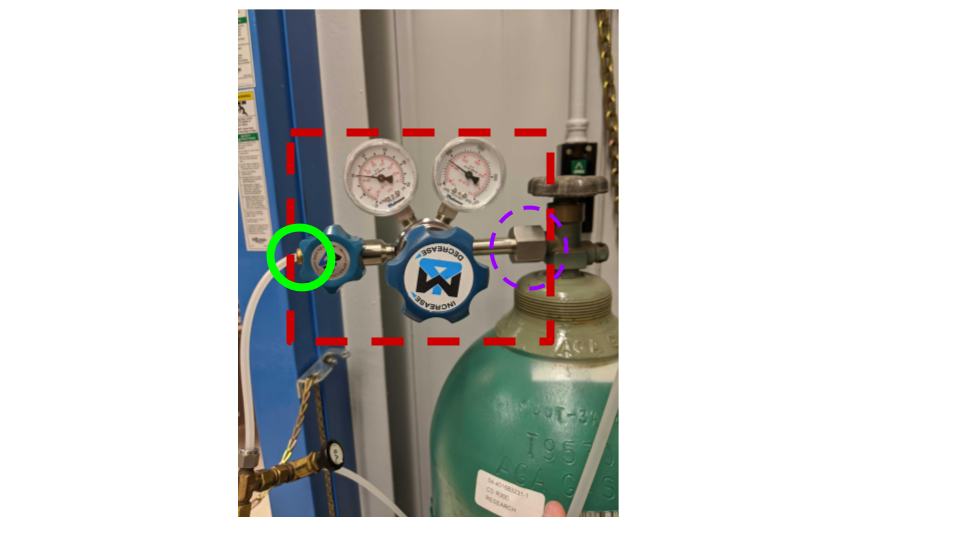
\includegraphics[scale=0.4]{DCT_gas_canister_example.png}
  \caption{The red dashed square outlines the gas regulator that needs attached to the canister. The purple circle outlines the output of the canister and input of the regulator. The green solid circle outlines the output of the regulator.}
  \label{fig:canister}
\end{wrapfigure}

The mixture is 90\% CO$_{2}$ and 10\% Ar. The outputs of each gas regulator is connected to the labelled inputs of the mixer. Make sure to level the mixer and see figure \ref{fig:mixer} for details.

\begin{figure}
  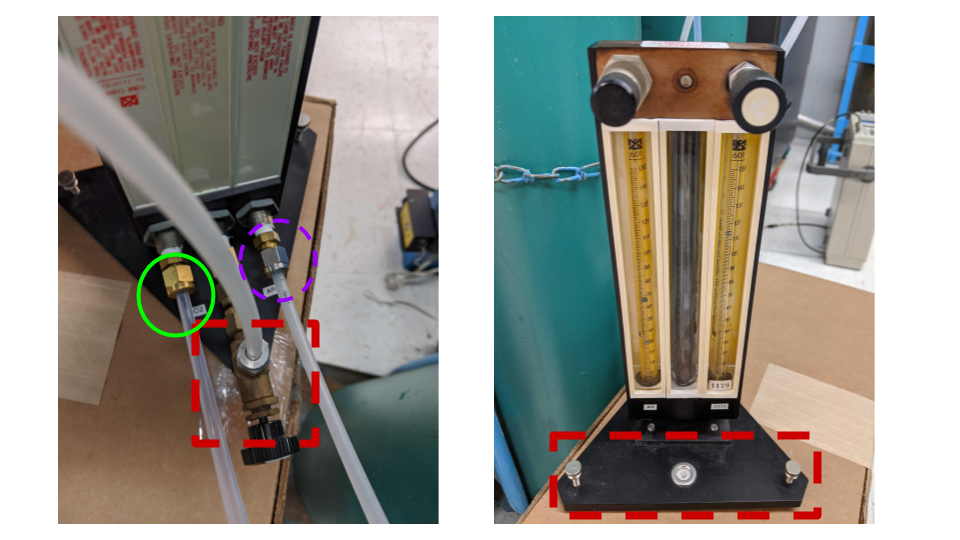
\includegraphics[scale=0.5]{DCT_gas_mixer_example.png}
  \caption{The back (left) and front (right) of the gas mixer. On the back, the red square shows the output of the mixer/mixed gas. The green solid circle shows the CO$_{2}$ input to the mixer and the purple dashed circle shows the Ar one. On the front of the mixer is clearly labelled the mix control of each gas type and the red dashed square shows the level and level-control of the mixer.}
  \label{fig:mixer}
\end{figure} %as a person who does not know much about the gas - Mixing ratio is controlled in here? What kind of control does this provide? What kind of mixing method is this one use?  
%answer: to acheive the 90-10 mixing ratio, the mixer manual needs to be referenced and has a setting based on the two floating bobs inside the levels. 

The output of the mixer goes through tubing to the input (west) side of the DCTV, clearly labelled in figure \ref{fig:DCTV_gas_input}. The DCT should be purged with this mixture in this setup for at least a day or two BEFORE turning on the HV of either the cathode or the potential wires. %question: what is the pressure setting for the purging? - Is the setting done at regulator for each gas canister or done at the mixer?
%answer: I need to go into more detail here to describe that. The mixer output is adjusted based on what makes the output look like its flowing but not too much flow. The regulator just needs to be open enough on each canister so we set them both at fully open and regulator at 2000 psi ~

\begin{figure}
  \centering
  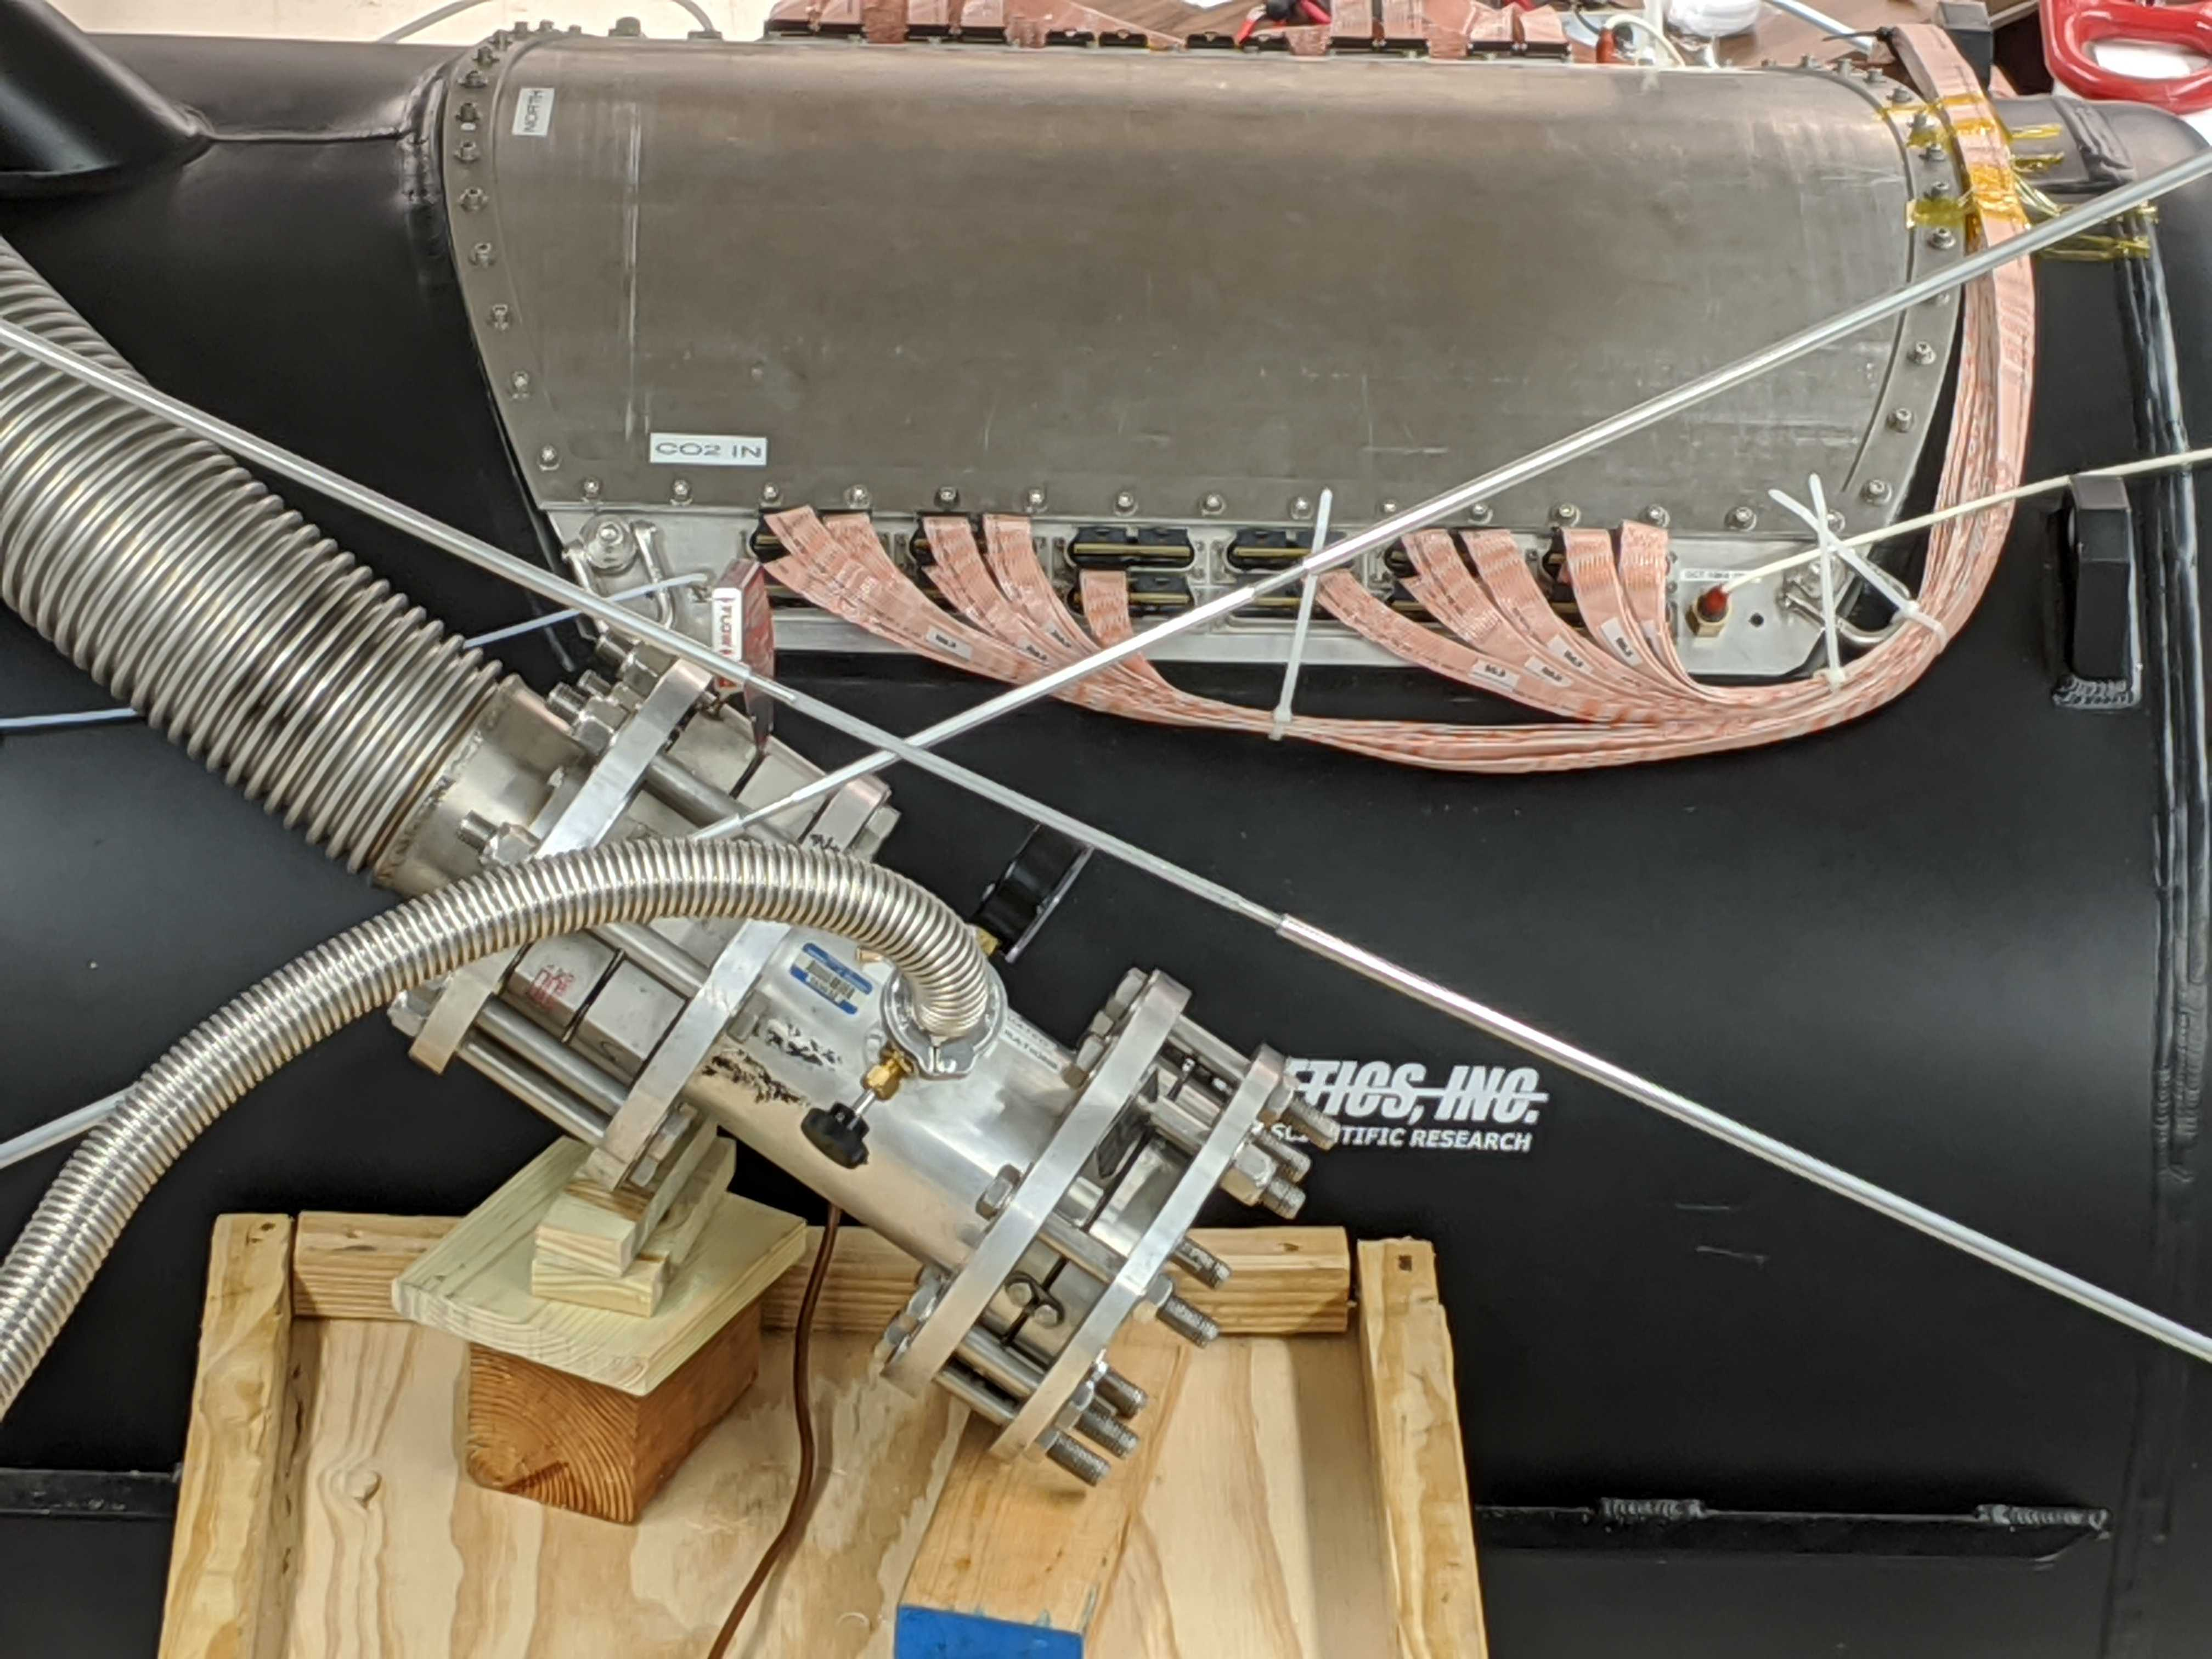
\includegraphics[scale=0.08]{DCT_gas_input.jpg}
  \caption{The west side of the DCTV with label "CO$_{2}$ IN" on the left with the tubing of gas connected. Also visible are the pre-amp cables out of the feedthroughs that go to the ADC boards.}
  \label{fig:DCTV_gas_input}
\end{figure} % hard to see the label with the size of the picture. Would you mind marking like you did for other pictures? I assume the white thin hose coming into the left side is the CO2 in. Is the right side white thin hose the CO2 out?
% answer: yes i can mark it. it is not very visible you are right.

\section{DCT NIM HV system setup}

Currently, we use the NIM HV supply provided by IU, appearing in figure \ref{fig:nim}. There are two sides to the supply, A and B. A is hooked up to the ``PTNTL'' wires (potential wires) and B is hooked up to the ``FIELD'' planes (field shaping wires). There are a number of things to check before turning on the supply. First, check the wiring to the supply and the DCTV labelling matches (potential or A is wired to potential port on the DCTV and the same for cathode or field to B). Next, check that the HV power switch and ``HV ON'' switches are off. Finally, reset the voltage dials to zero on both sides of the supply and set the current trip switches to ``auto''. 

\begin{wrapfigure}{C}{6cm}
  \hspace{-1.4in}
  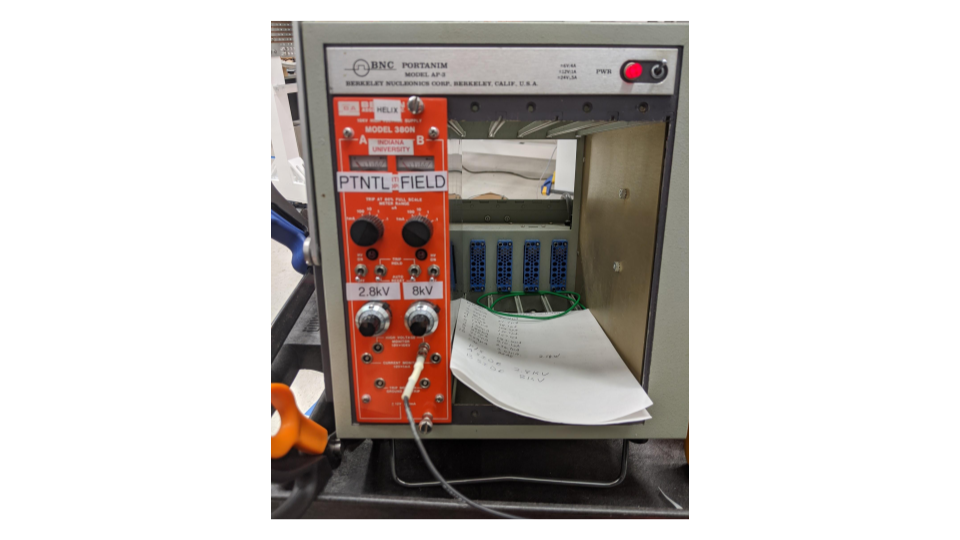
\includegraphics[scale=0.4]{dct_nim_Hv.png}
  \caption{The HV supply we use currently is the NIM one here, with two different outputs labelled as ``FIELD'' and ``PTNTL''. One of the LEMO ports is being used in this picture on the B side.}
  \label{fig:nim}
\end{wrapfigure}

Remember, the current trip settings on the NIM supply are 80 \% of the trip dial setting. Therefore, a current trip of 1~$\mu A$ on the supply will trip instead at 0.8$~\mu A$. The following current trip settings are current as of 02/24/2020: potential wires should have a current trip of $1$~uA and the cathode plane has $1$~mA. 

Once the current trip settings are correct, turn on the power and the HV switches of both sides. Immediately switch on the trips to ``trip hold'' (this stops the supply from resetting to the previous voltage when a trip occurs). The red lights on each side should be on now. If they are not, stop it and check stuff. 

\section{Ramping Up}
DO NOT RAMP UP UNLESS THE DCT HAS BEEN PURGED WITH CO$_{2}$ MIXTURE AND EVEN THEN RAMP UP SLOWLY IF IT IS FIRST TIME RAMPING SINCE PURGE.

ALWAYS RAMP UP THE CATHODE PLANES FIRST TO $6$~kV, THEN THE POTENTIAL TO $2$~kV AND WAIT A LITTLE (5 MINS). % Do you start the ramping up by setting the cathode plane first to 6 kV? Or do you slowly ramping up to 6 kV?  Is the cathod planes to 6 kV / potential to 2 kV is the final HV set you want to put on? 

%answer: this needs to be described better. Ramping up should be done 'cautiously' but there is not set speed. Its basically just slow enough to watch the currents not rise too fast because then you risk tripping the HV supply and have to start over. Also 6,2 is not the final state just the one we hold the chamber at for a while before going to 'full field' or operating potentials.

The chart below shows the current reading at each voltage reading that should roughly be observed if the DCT is feeling good. 

\begin{tabular}{|c|c|} \hline
    V(kV) & I($\mu$A) \\\hline
    1 & 25.4 \\
    2 & 51.7 \\
    3 & 78.1 \\
    4 & 104.3 \\
    5 & 130.7 \\
    6 & 157.1 \\
    7 & 183.6 \\
    8 & 210.1 \\
    9 & 236.7 \\
    10 & 263 \\\hline
\end{tabular}

This supply has 2 BNC ports on each side (A and B), one for Voltage and one for current. Connect a multi-meter to the voltage LEMO port of the side being ramped to read the voltage of the supply (divided by $1000$). The current port is read with a multi-meter as well. The potential wires should read very close to 0 amps throughout the ramping (ya know, $>200$~G\ohm). % you mean, multi-meter?, yes!

\section{Flight HV supply}
The UM8-40 spellman HV supply is the chosen supply for flight. It had corona issues, was placed into a box and shielded in mu-metal. Good grief. 

For flight, we will use a current limit on the cathode plane of $400$uA. 

\section{Assessing the integrity of the DCT}
We use a ``Keithley 6514 System Electrometer'' to gauge the resistance of the DCT, the field resistance and the potential resistance. The field resistance should read out at $38$~M\ohm. The potential wire should read off the scale ($>200$~G\ohm). Hook these up with ground of ohmeter to ground line and the input line to the positive of the ohmeter. % is there particular ohmeter used for this? Or regular multi-meter works?
%answer: need to use an electrometer that can read these resistances this high so we use this electrometer religiously, but its not apparent if another would be better/worse because they have never used another one as far as I am aware. s

If the DCT+V has not been purged with gas, the reading on the potential wires will be lower. %how much lower? - 50 GOhm is the lowest you expect to see? Or can be lower? 
%correct, probably about 50Gohm but not much lower than that I assume. 
It has been observed to increase slowly to off the scale ($>2$~days) from below $50$~G\ohm. Side-by-side picture of the reading on the potential wires with the electrometer is shown in figure \ref{fig:electrometer}. The typical test of DCT health before ramping up is to observe these resistances. It takes a long time for the electrometer to reach off the scale readings on the potential wires ($>1$~hour). %it will be nice if you can list a particular symptom for known issues. Say, if I read lower than xxx resistance value, what does that tell me? If the resistance does not increase to off the scale within 2 days, what does that mean? 
%Answer: yes I will. 

\begin{figure}
  \centering
  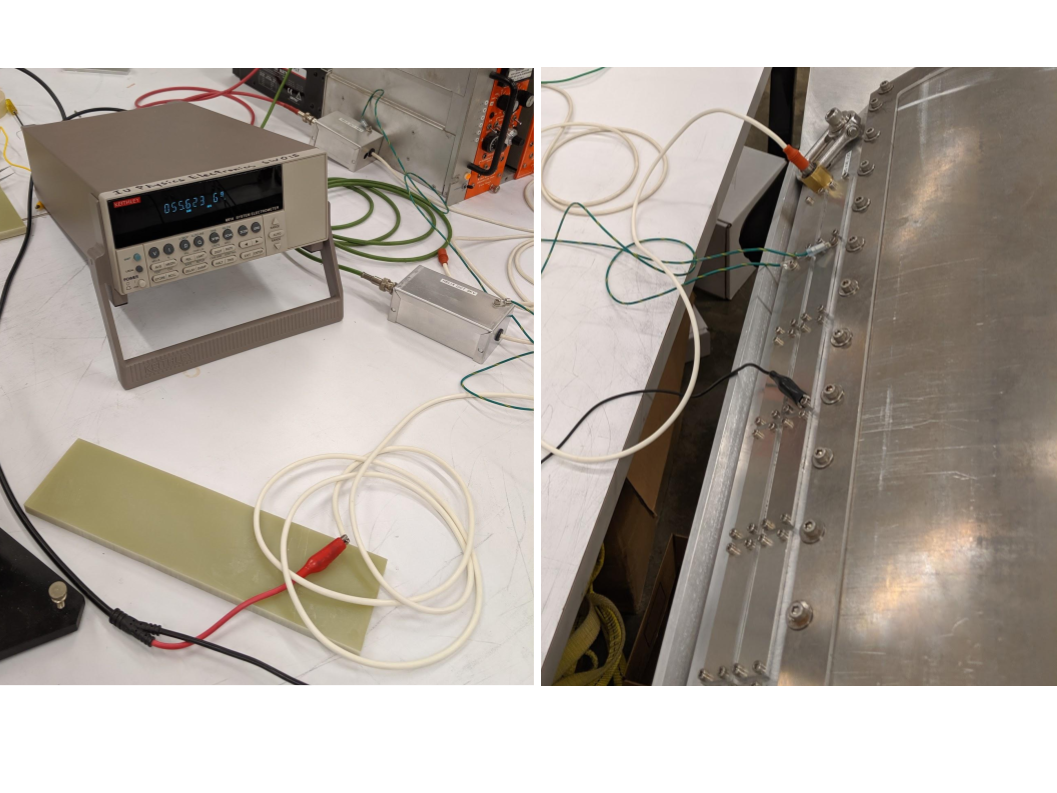
\includegraphics[scale=0.4]{DCT_keithley.png}
  \vspace{-0.4in}
  \caption{The electrometer hooked up to the potential port of the DCTV lid and reading out at $50$~G\ohm.}
  \label{fig:electrometer}
\end{figure} % what is each wire? I assume black one is the ground, white cable is the potential port - meaning that it is reading out the HV applied to the potential wires? What is the green wire?
%answer: green is the ground of the cathode here. I will list it. 
\section{Wire, Motherboard, and Pre-amp board mapping}

There are 18 motherboards on each side of the north and south of the DCT, for a total of 36. %How this North and South in the magnet coordinate? - see the wiki page for the coordinate definition in HELIX: http://helix.uchicago.edu/wiki/pmwiki.php?n=Simulations.HomePage
%answer: it is in those coordinates where north is stack, as viewed from above the magnet looking down out at it. 
A pre-amp board is attached on top of one half of these boards (the half with pins for the sense wires). The Motherboards for the north and south side are slightly different but the pre-amp boards are identical for both sides. In both figure \ref{fig:North} and \ref{fig:South}, motherboards are shown at the top left and a pre-amp board is shown in figure \ref{fig:Pre-amp}. On each pre-amp board is an IDC connector that takes the differential pair output of the twelve sense wire signals (after conversion to voltage and amplification, so total of 24 channels) to a feedthrough port on the DCTV lid. %just to be sure, so the mother board numbering & preAMP numbering is 1:1 matching? Say, Fig8's feedthrough labeling is preAMP labeling, and it would match with the corresponding mother board labeling shown in figure 6?
%answer: yes that is correct, each motherboard has a preamp board on top of it and therefore the pre-amp cables are labelled by the motherboard labels so it is def 1:1.
The north and south motherboards are different by a mirror reflection across the wires, such that the signal pins are to the left of the wires on a north motherboard and are to the right of the wires on a south motherboard. 

Each motherboard+pre-amp board has a label according to its side (N/S) and its position from the top to the bottom. This is shown in both figures \ref{fig:North} and \ref{fig:South}. The labelling is such that N1.1 and S1.1 are both the top-east board position. This is done so that the same label board is used on each side of the same wire hence the labels are mirrored. Per motherboard the wires are also labelled as channels from top to bottom: ${0,11}$. A sense wire is read as having a north side label N1.10 which is channel 0 or the top sense wire of board N1.1 and that same sense wire has a south side label of S1.10.

\begin{figure}
\label{fig:exp}
\begin{subfigure}{.45\textwidth}
    \centering
    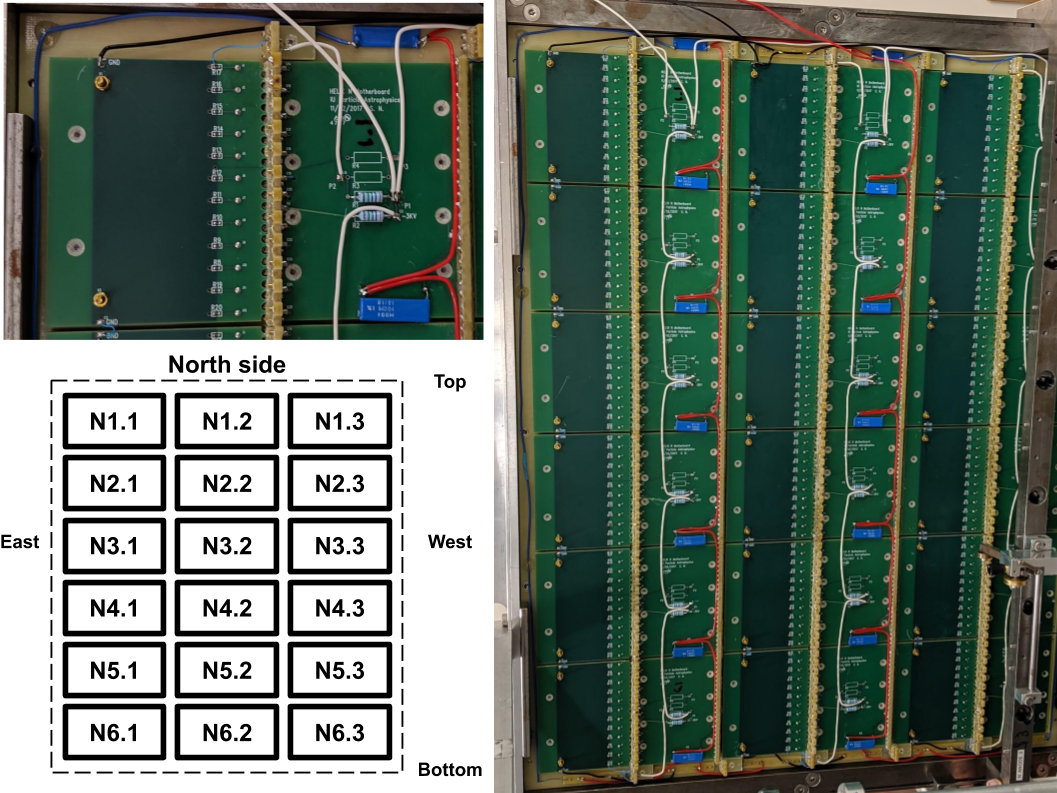
\includegraphics[scale=0.2]{DCT_N_side_mb_labels.png}	\vspace{0.1in}
    \caption{The North side of the DCT with motherboards (green) visible and wire pins exposed. The labelling of each board position is shown to the left and a single motherboard is shown at the top left.}
    \label{fig:North}
\end{subfigure}\hspace{0.05\textwidth}%
\hspace*{\fill} % separation between the subfigures
\begin{subfigure}{.45\textwidth}
  \centering
  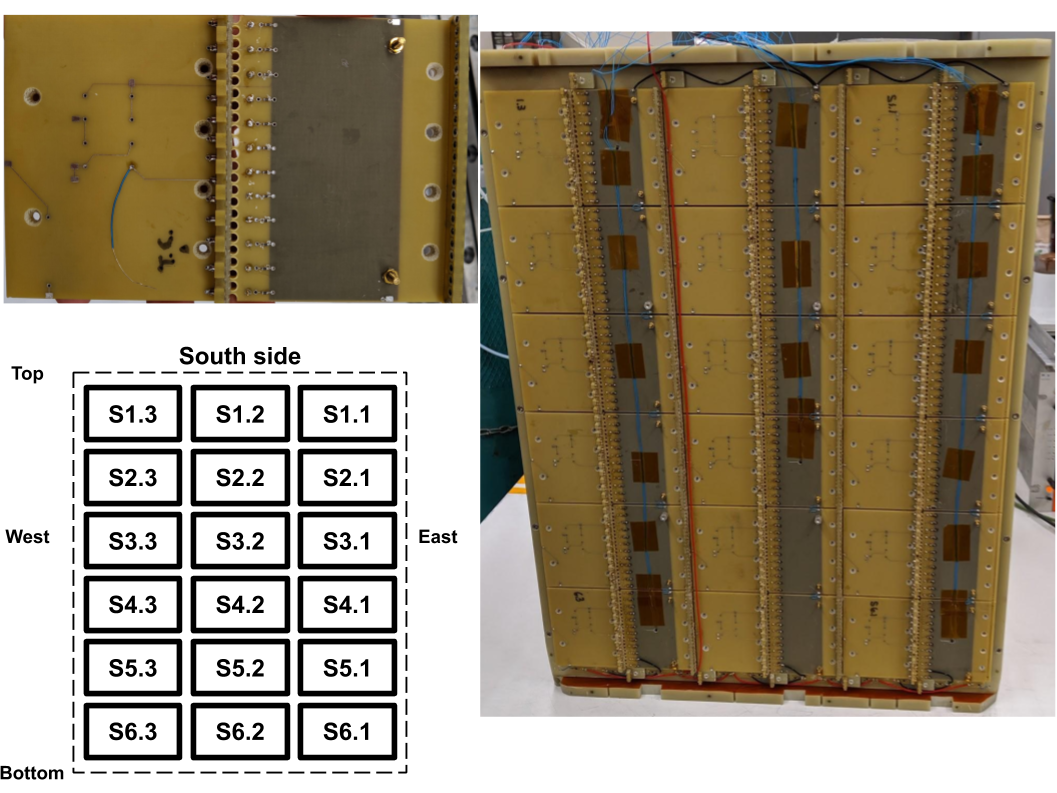
\includegraphics[scale=0.2]{DCT_S_side_mb_labels.png}
  \caption{The South side of the DCT with motherboards (G10 gross color) wire pins visible. The labelling of each board position is shown to the left and a single motherboard is shown at the top left.}
  \label{fig:South}
\end{subfigure}
\vspace{-0.1in}
\caption{DCT North and South side legends and motherboard examples.}
\end{figure}

The pre-amp cables inside of the DCTV connect to feedthrough boards. The feedthrough boards have two ports each and an example with a cable is shown in figure \ref{fig:board}. Through the feedthroughs and out of the DCTV, the cables trace around the gondola to the ADC boards that are positioned in a crate on the southeast corner of the magnet.
An ADC board takes 4 pre-amp connectors, so that means there are 48 sense wires with 96 channels to read per ADC board. Here it is important to note that each sense wire is read out on both sides. Thus, there are 48 sense wires per ADC board and 9 total ADC boards, which would give 432 sense wires however half of these are the other side of the sense wires, so there are only 216 sense wires. But, the pre-amp boards output differential pairs, so there are really 864 channels in total read from the DCT. A picture is shown with labels on each feedthrough so we know which board (and hence which wire) is reading out on the channel of each ADC board. The cables are unique lengths such that the motherboard to ADC board distance of cable is the same for all cables. This requires unique positions for each pre-amp cable on the DCTV feedthroughs and can be seen with the labels in figure \ref{fig:legend}. 

\begin{figure}
  \centering
  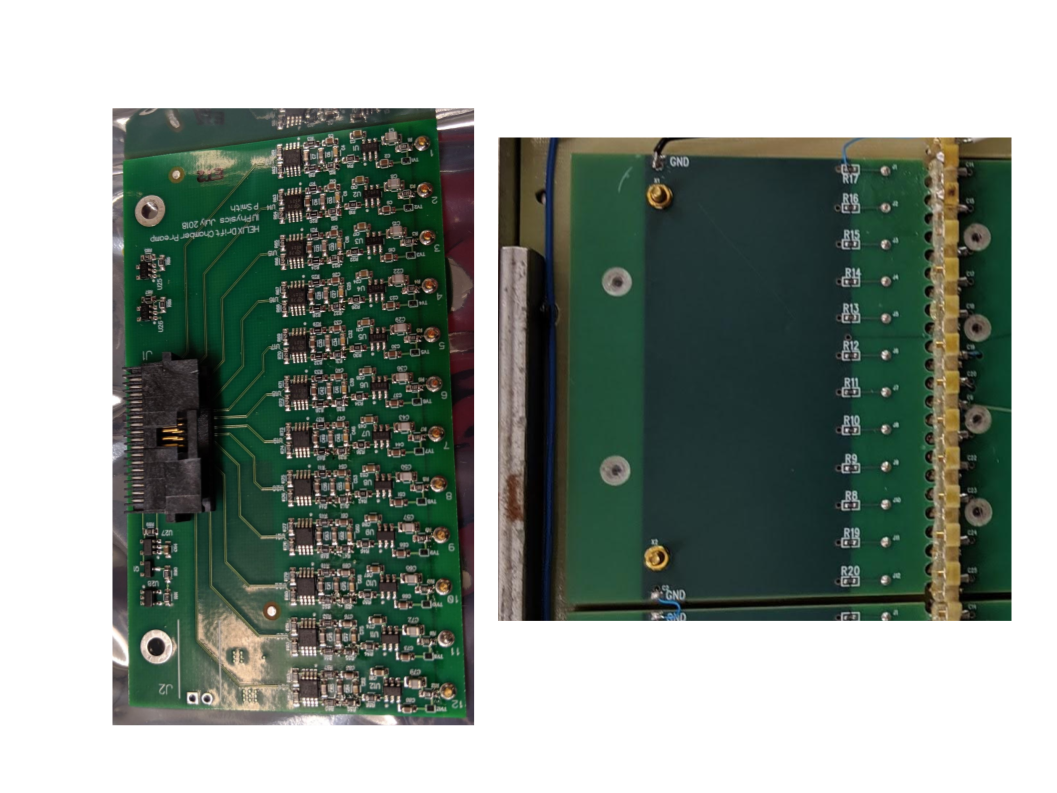
\includegraphics[scale=0.25]{DCT_Preampboard.png}
  \caption{A pre-amp board on the left and half of a motherboard on the right. The right edge of the pre-amp board has the pin covers visible that electrical connect to the pins on the mother board, which are to the left of the wires but to the right of the ground plane. The screw ends sticking out of the left of the motherboard fit through the holes on the left edge of the pre-amp board, and nuts are used to secure them together electrically and mechanically.}
  \label{fig:Pre-amp}
\end{figure}


\begin{figure}
  \centering
  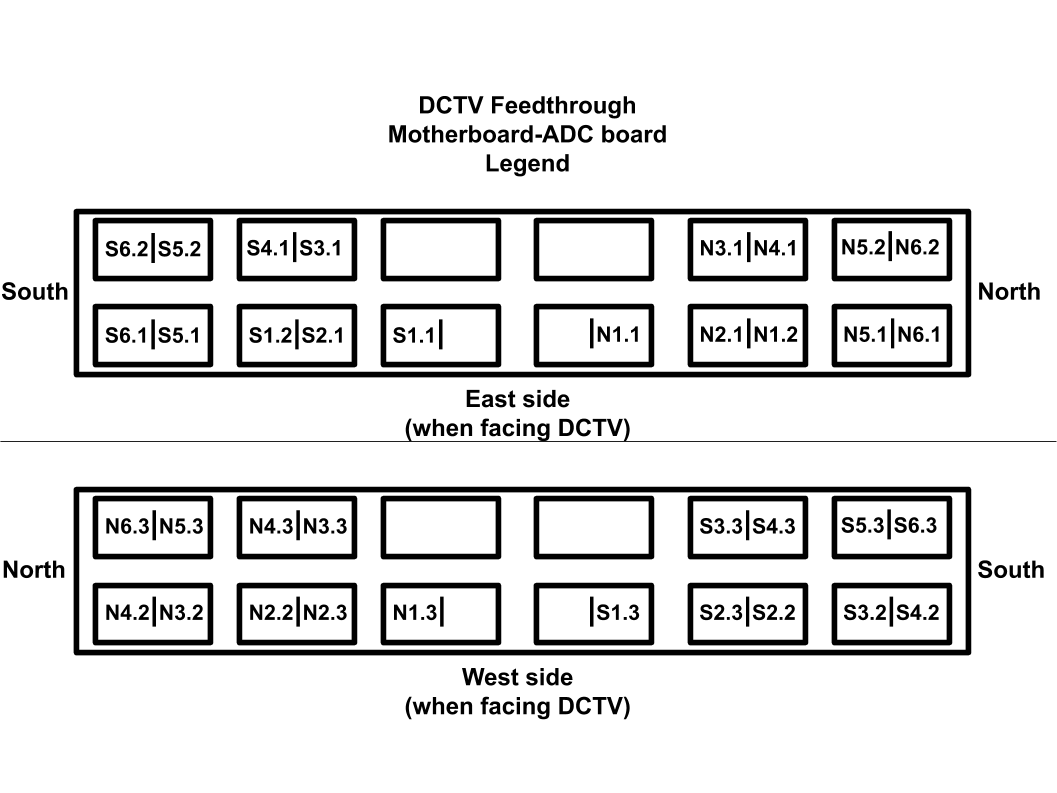
\includegraphics[scale=0.25]{DCT_feedthrough_legend.png}
  \caption{Legend showing the DCTV lid (both sides) with feedthrough ports labelled by pre-amp board cables.}
  \label{fig:legend}
\end{figure}


\section{DCT HSK}

There are 24 thermistors that are out of two of the feedthroughs from the DCTV lid. They are in positions blah and blah. %fill in the 'blah' when you know the details  :)
The other positions are described in the ADC feedthrough section. The thermistors are labelled based on their position on the DCT, with 5 on each of the North, South, East and West sides and 2 on each of the top and bottom. They are read in using LTC2983 chips that convert their resistance readings as ratio to a precisely known sense resistor. This resistance is then converted to a temperature using the Thermistors specific Steinhart-Hart approximation. This calculation is done on the chip before being read in by the DCT sub-housekeeping board.


\begin{wrapfigure}{R}{6cm}
  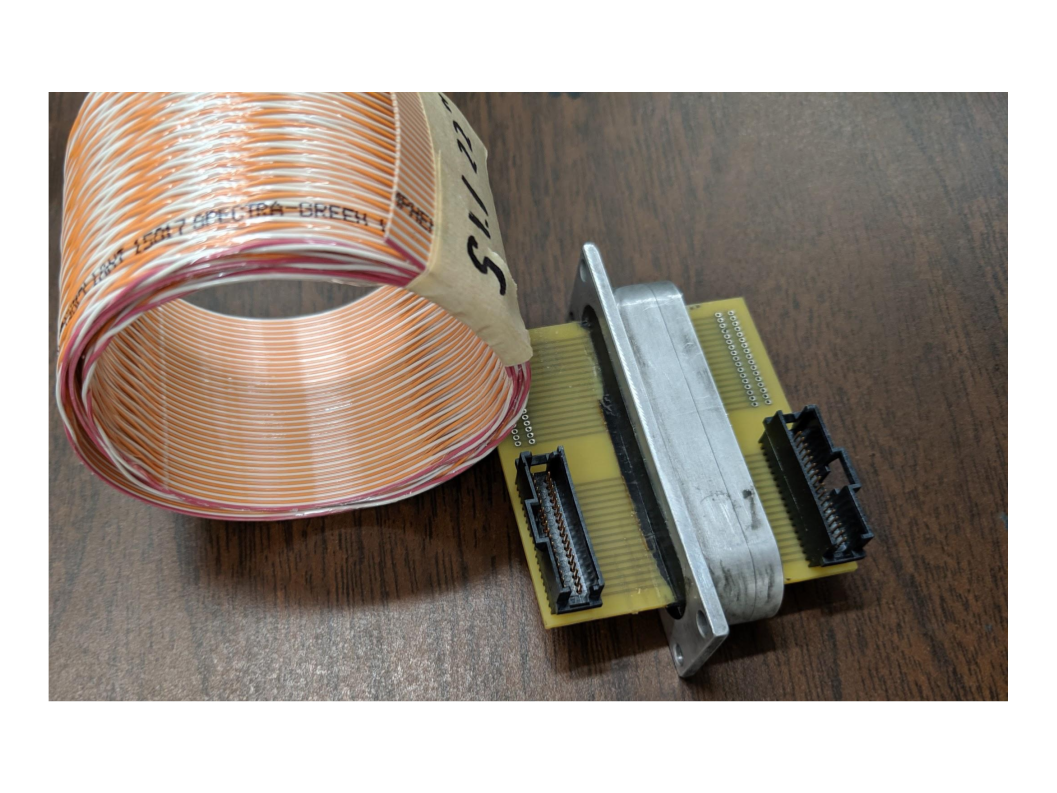
\includegraphics[scale=0.2]{DCT_feedthrough.png}
  \caption{A feedthrough board epoxied to a feedthrough with two IDC connector footprints visible along with an internal cable for motherboard-to-feedthrough connection.}
  \label{fig:board}
\end{wrapfigure}
\end{document}
